%
% teil3.tex -- Beispiel-File für Teil 3
%
% (c) 2020 Prof Dr Andreas Müller, Hochschule Rapperswil
%
% !TEX root = ../../buch.tex
% !TEX encoding = UTF-8
%
\section{Rekonstruktion eines CT-Scans
\label{ct:section:rekonstruktion}}
\rhead{Rekonstruktion eines CT-Scans}
Im letzten Abschnitt über die Rekonstruktion von CT-Bildern wird untersucht, wie Röntgendaten in klare und aussagekräftige Bilder umwandelt werden. Dabei werden die zwei wichtigen Theoreme das Zentralschnitt-Theorem und die gefilterte Rückprojektion nochmals angewendet. In diesem Abschnitt wird ein praktisches Beispiel für die Rekonstruktion von CT-Bildern verwendet, um diese Theoreme in der Praxis zu veranschaulichen. 

\subsection{Das Beispiel
\label{ct:subsection:malorum}}
Als einfaches Beispielbild werden zwei Kreise in der Ebene verwendet, siehe Abbildung \ref{ct:img_example}. So bleibt auch das radontransformierte Bild übersichtlich.

\begin{figure}
	\centering
	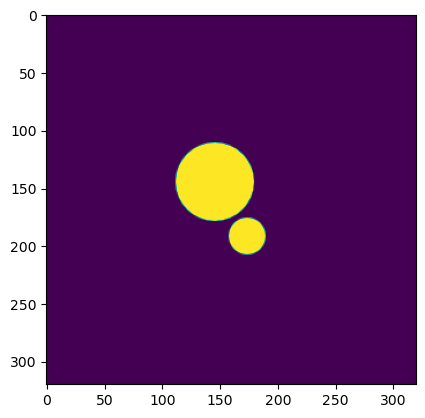
\includegraphics[width=0.5\linewidth]{papers/ct/images/img_recon.png}
	\caption{Das Beispielbild
		\label{ct:img_example}}
\end{figure}

Die Rückprojektion in der Praxis verwendet nur eine endliche Anzahl von Werten. Dies führt dazu, dass die Rückprojektion nicht mit einem Integral berechnet werden kann, sondern mit einer Summe approximiert werden muss. 
Die kontinuierliche Variable $\theta$ wird in der diskreten Umgebung der Rückprojektion mit der diskreten Variable $\theta_i$, die sich auf die Winkel ${k\pi/N: 0\le k \le N-1}$ beschränkt, ersetzt. Diese Diskretisierung wird mit 
\begin{equation}\label{ct:discreteBP}
		\mathscr{B}_Dh(x, y) = \big(\dfrac{1}{N}\big)\sum_{k=0}^{N-1} h(x\cos(k\pi/N)+Y\sin(k\pi/N), k\pi/N)
\end{equation}
beschrieben, wobei $k\pi/N$ mit $\theta_i$ zur Übersichtlichkeit ersetzt werden kann und somit resultiert
\begin{equation}\label{ct:discreteBP}
	\mathscr{B}_Dh(x, y) = \big(\dfrac{1}{N}\big)\sum_{k=0}^{N-1} h(x\cos(\theta_i)+y\sin(\theta_i), \theta_i).
\end{equation}

Das Bild, welches vom Scanner erhalten wird, wird in \ref{ct:img_radon} gezeigt.
\begin{figure}
	\centering
	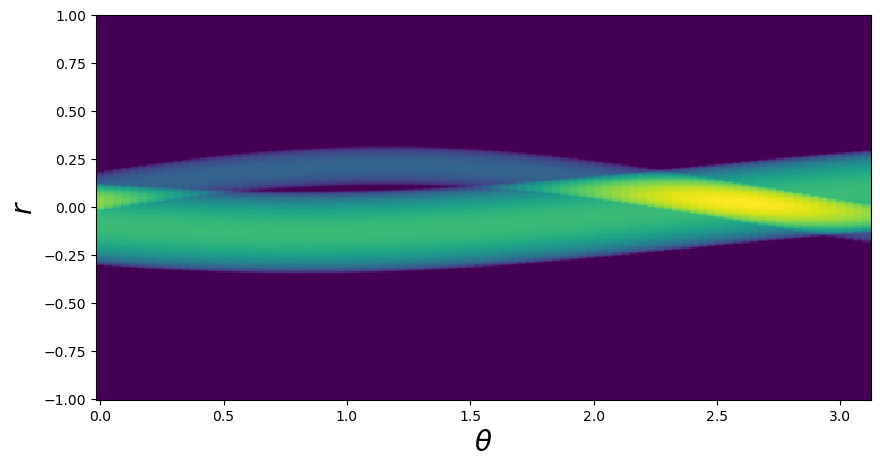
\includegraphics[width=0.5\linewidth]{papers/ct/images/radon.png}
	\caption{Die Radon-Transformation des Beispielbildes.
		\label{ct:img_radon}}
\end{figure}

Auf das Bild vom Scanner wird zunächst die Rückprojektion angewendet. Dies führt dazu, dass das Bild eine \glqq geglättete\grqq{} Version des Beispielbildes wird. Dies wird in der Abbildung \ref{ct:img_bp} gezeigt.
\begin{figure}
	\centering
	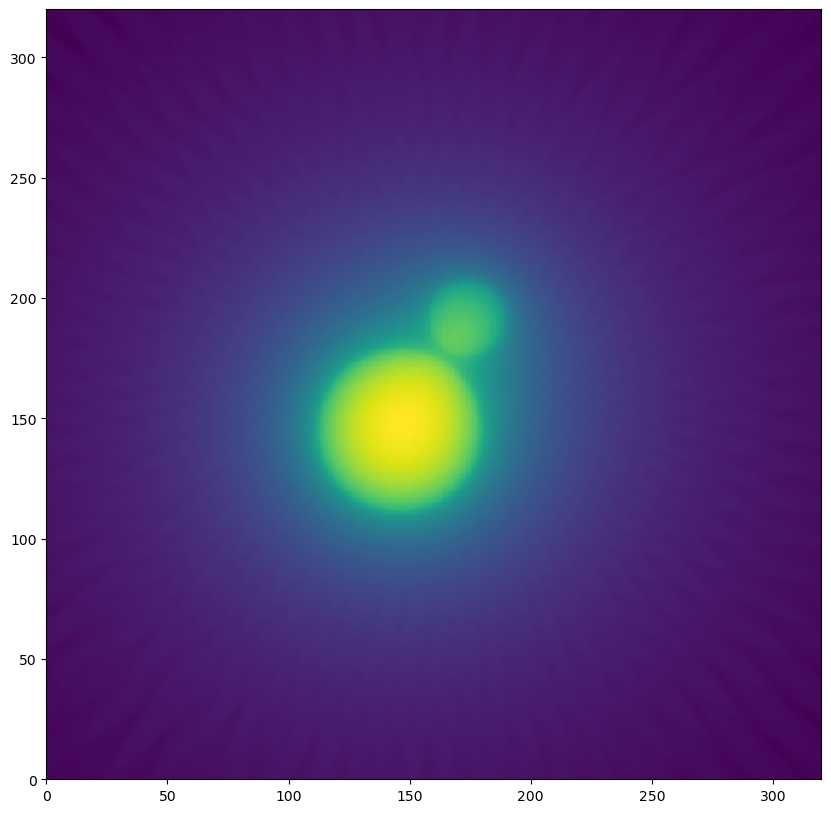
\includegraphics[width=0.5\linewidth]{papers/ct/images/bp.png}
	\caption{Die Rücktransformation des Beispielbildes.
		\label{ct:img_bp}}
\end{figure}

Damit ein ungeglättetes Bild resultiert, wird die gefilterte Rückprojektion angewendet. Dabei wird als erstes, Abbildung \ref{ct:img_radon} Fourier-transformiert. Danach wird die Filterung mit $|S|$ durchgeführt und die inverse Fourier-Transformation wird gebildet. Schliesslich wird noch die Rückprojektion durchgeführt, was zur gefilterten Rückprojektion führt. 

\begin{figure}
	\centering
	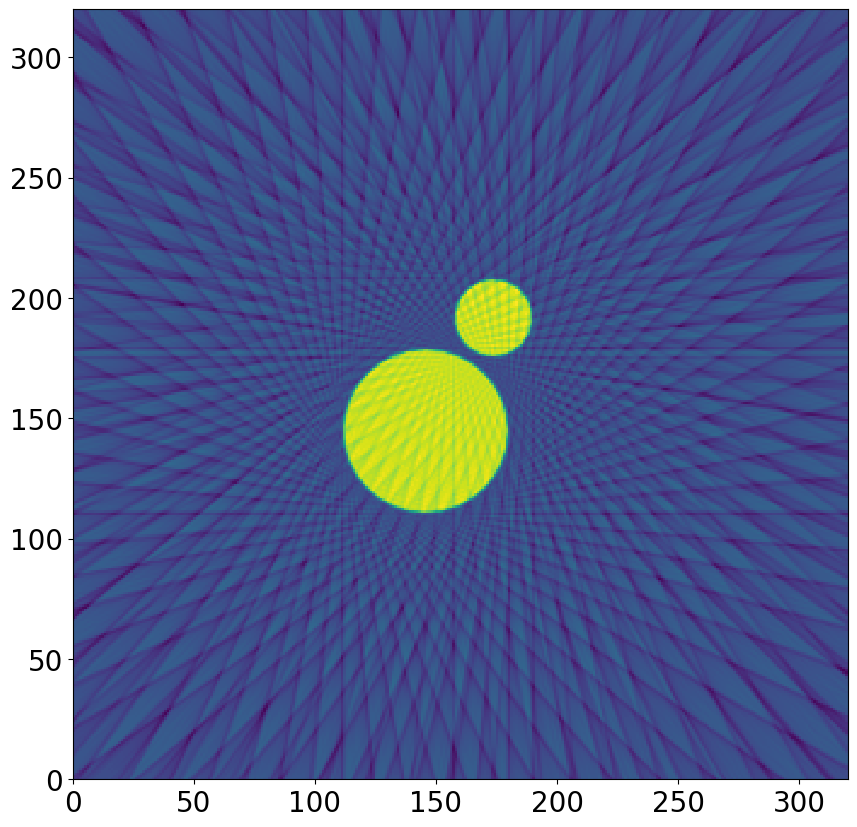
\includegraphics[width=0.5\linewidth]{papers/ct/images/fbp.png}
	\caption{Die gefilterte Rücktransformation des Beispielbildes.
		\label{ct:img_fbp}}
\end{figure}

Im Bild kann man noch gewisse Artefakte sehen, die sich durch Linien im Bild zeigen. Diese Artefakte kommen daher, dass die Winkelauflösung begrenzt ist. In der Abbildung \ref{ct:img_resol} werden noch zwei Rekonstruktionen gezeigt, die einerseits eine tiefere Winkelauflösung und andererseits eine noch höhere Auflösung darstellen.

\begin{figure}
	\centering
	\begin{minipage}{0.45\linewidth}
		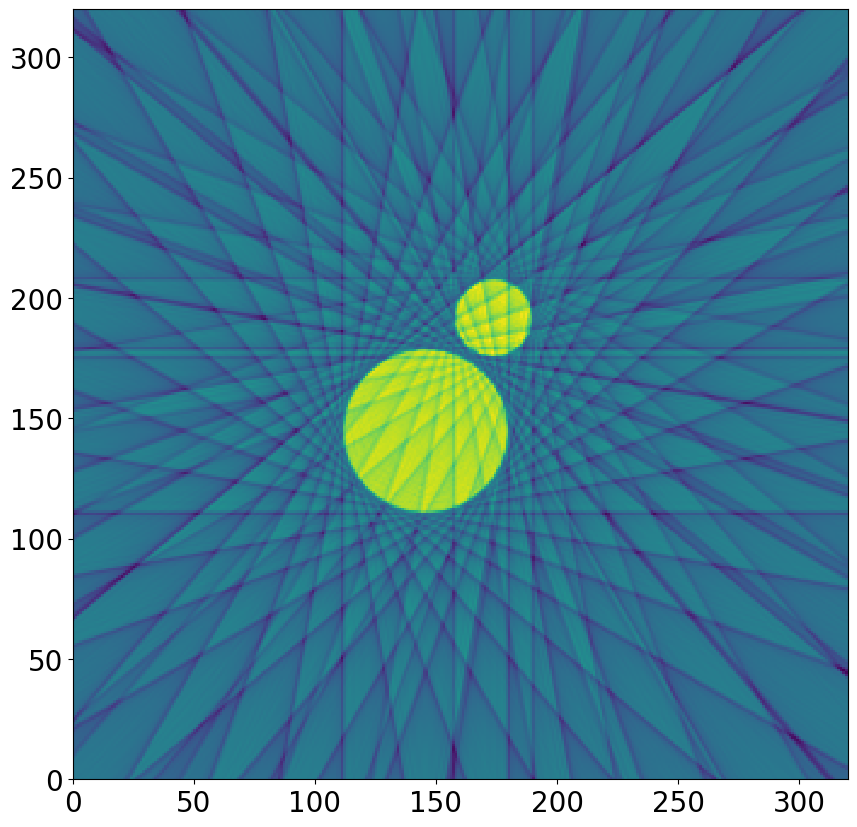
\includegraphics[width=\linewidth]{papers/ct/images/fbp_low.png}
	\end{minipage}
	\begin{minipage}{0.45\linewidth}
		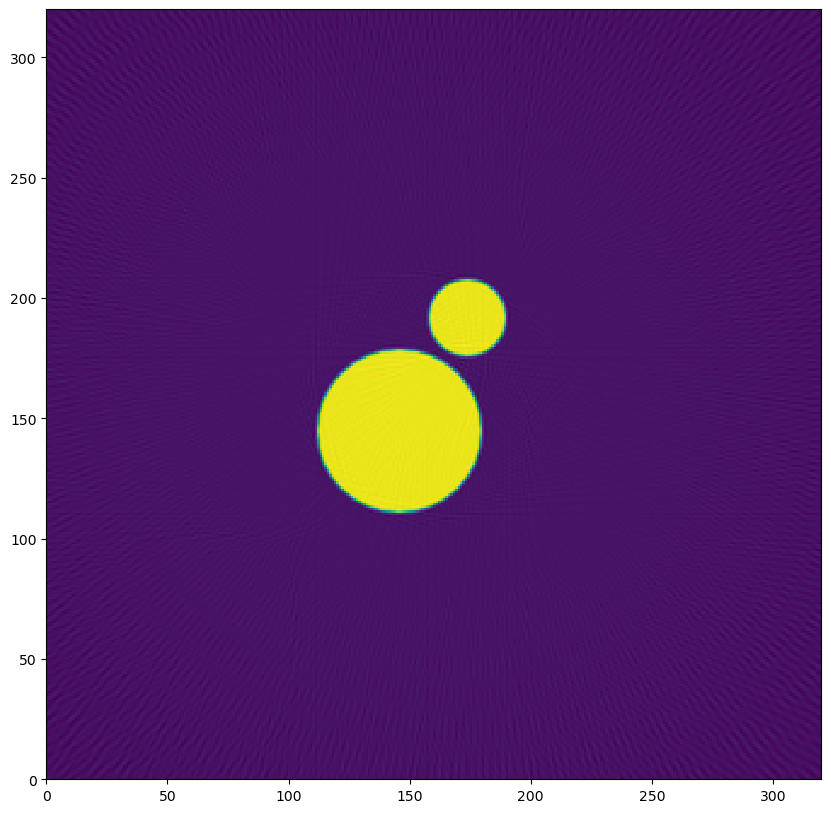
\includegraphics[width=\linewidth]{papers/ct/images/fbp_high.png}
	\end{minipage}
	\caption{Die gefilterte Rücktransformation mit 10° (links) und 1° (rechts) Winkelauflösungen.
	\label{ct:img_resol}}
\end{figure}










